\section{Fundamento teórico}



%%%%%%%%%%%%%%%%%%%%%%%%%%%%%%%%%%%%%%%%%%%%%%%%%%%%%%%%%%%%%%%%%%%%%%%%%%%%%%%%
\begin{frame}
\frametitle{\citetitle{kreiss2019pifpaf}}
Convolutional: Resnet, Part Intensity Fields (PIF), Part Association Fields (PAF)
\begin{figure}[h!]
\centering
\includegraphics[width=0.65\linewidth]{images/soccer.jpeg.predictions.jpeg}
\caption{Pontos-chave superpostos na imagem (Fonte: Website de OpenPifPaf \cite{kreiss2019pifpaf})}%kreiss2019pifpaf %OpenPifPaf
\label{fig:soccer.predictions}
\end{figure} 
\end{frame}

\begin{comment}
\begin{frame}
    \frametitle{\citetitle{kreiss2019pifpaf}}
    \begin{figure}[h!]
    \centering
    \includegraphics[width=0.95\linewidth]{images/openpifpaf.png}
    \caption{Diagrama do sistema (Fonte: Website de OpenPifPaf \cite{kreiss2019pifpaf})}%kreiss2019pifpaf %OpenPifPaf
    \label{fig:soccer.predictions}
    \end{figure} 
    \begin{figure}[!hbt]
        \centering
          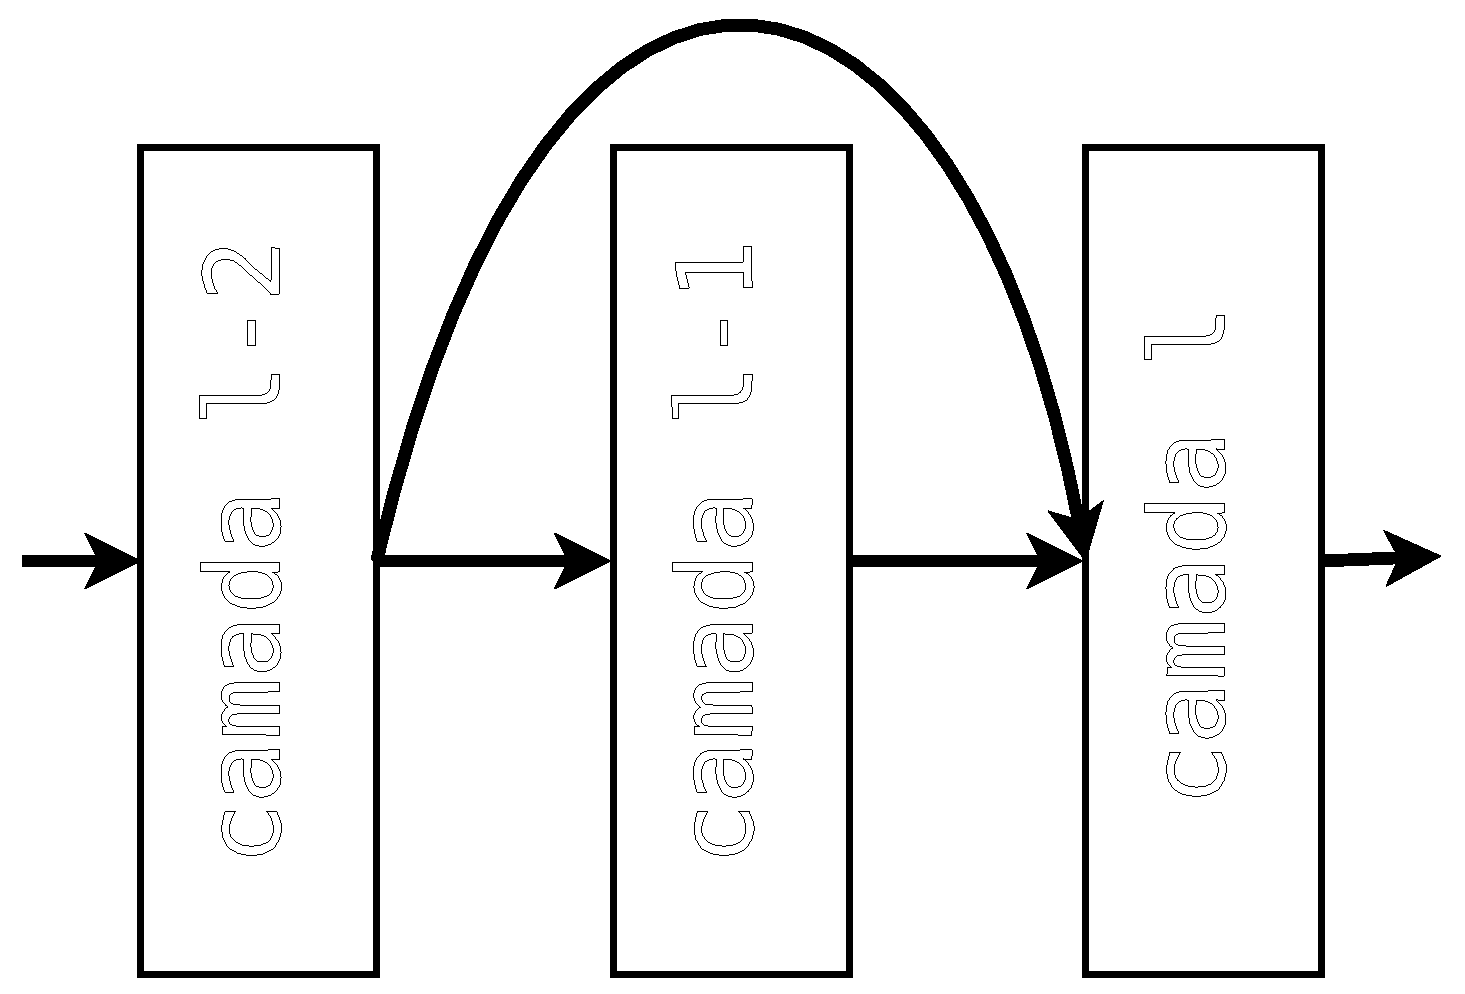
\includegraphics[width=0.25\textwidth]{images/residual.eps}
          \caption{Camadas com informação residual.}
          \label{fig:residual}
    \end{figure}
\end{frame}
\end{comment}

%%%%%%%%%%%%%%%%%%%%%%%%%%%%%%%%%%%%%%%%%%%%%%%%%%%%%%%%%%%%%%%%%%%%%%%%%%%%%%%%
\begin{frame}
    \frametitle{CNN 2D}
    Conv2D, MaxPooling, Dropout, Flatten, BatchNormalization, Dense, etc.
    \begin{figure}[h!]
    \centering
    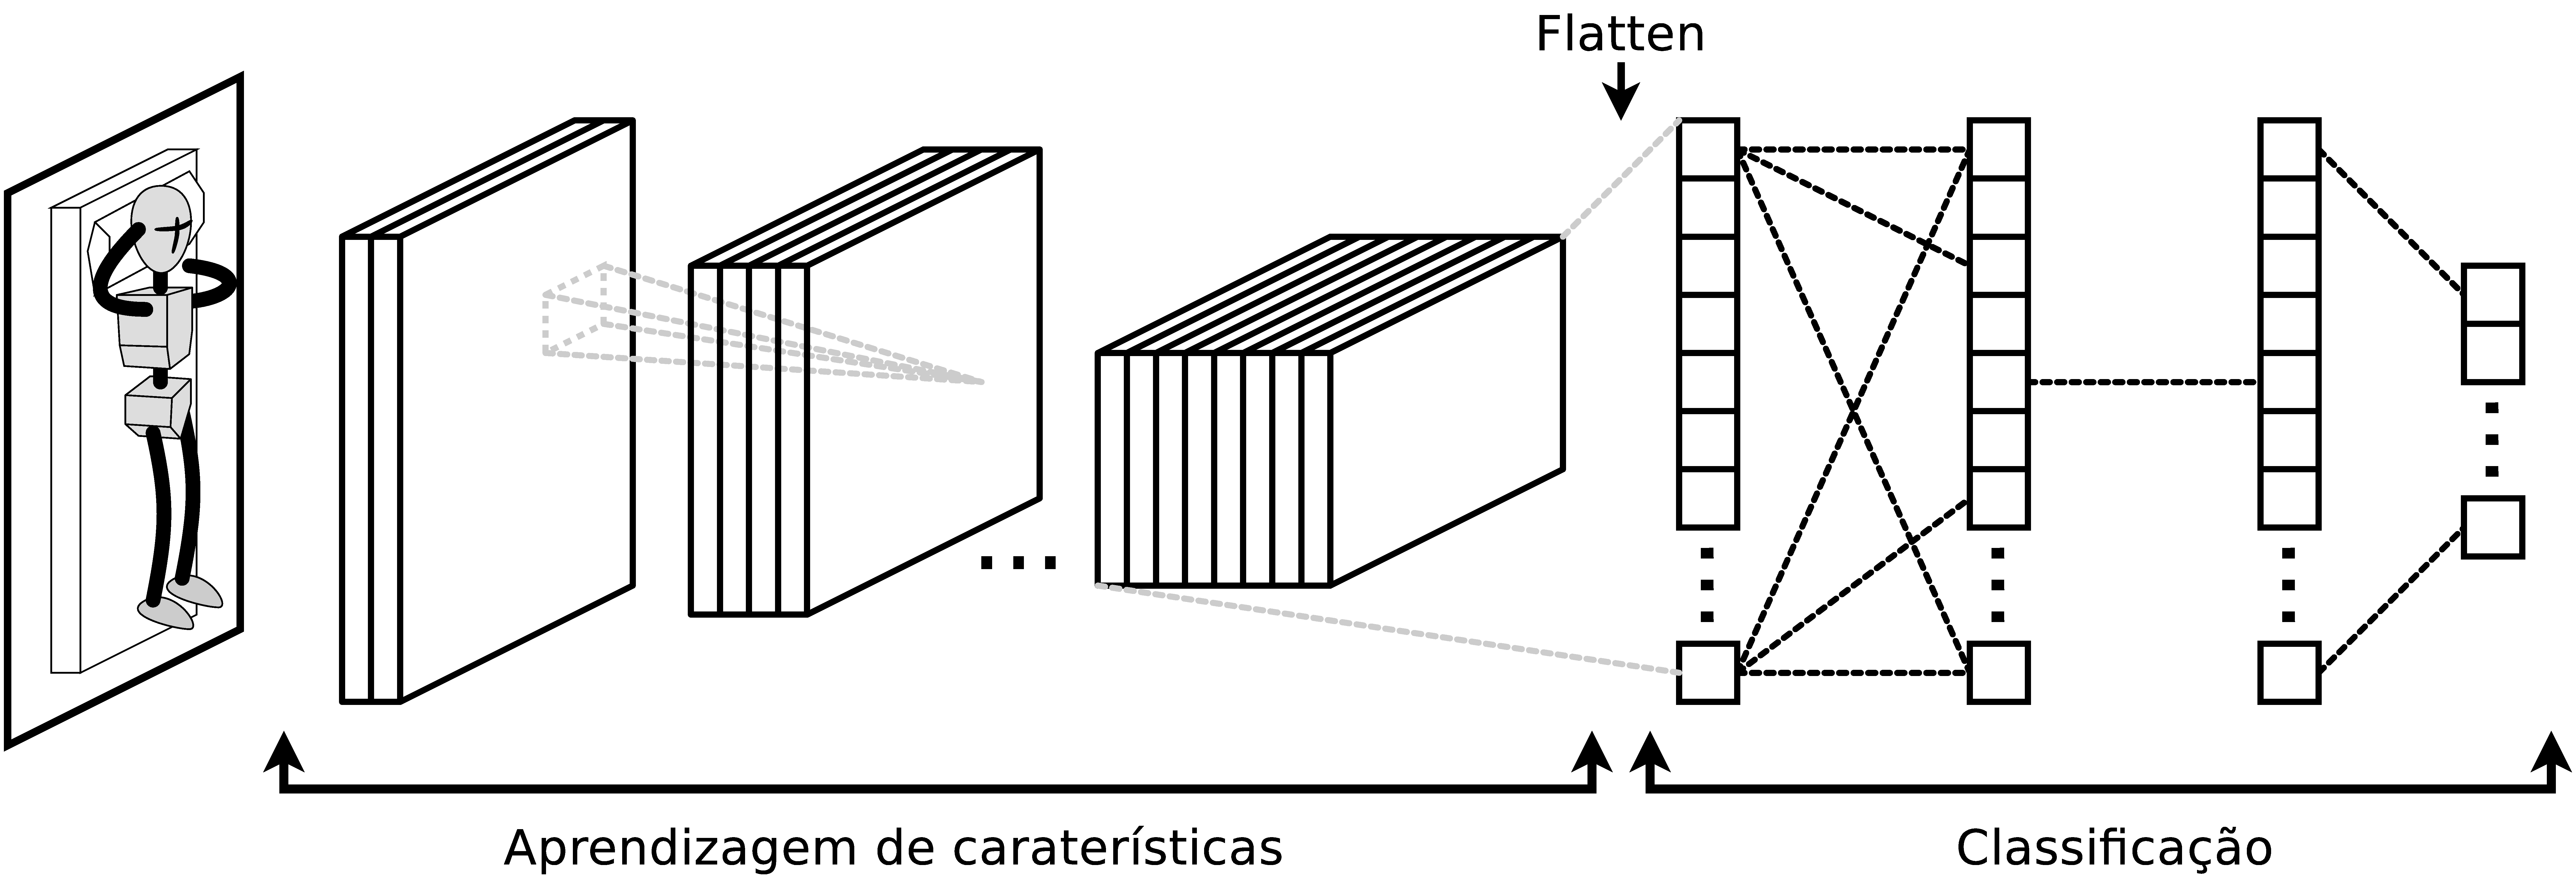
\includegraphics[width=0.75\linewidth]{images/body-image.eps}
    \caption{Rede neuronal convolucional (Fonte: Autor)}%kreiss2019pifpaf %OpenPifPaf
    \label{fig:body-image}
    \end{figure} 
\end{frame}

%%%%%%%%%%%%%%%%%%%%%%%%%%%%%%%%%%%%%%%%%%%%%%%%%%%%%%%%%%%%%%%%%%%%%%%%%%%%%%%%
\begin{frame}
    \frametitle{Fusão tardia}
    \begin{figure}[h!]
    \centering
    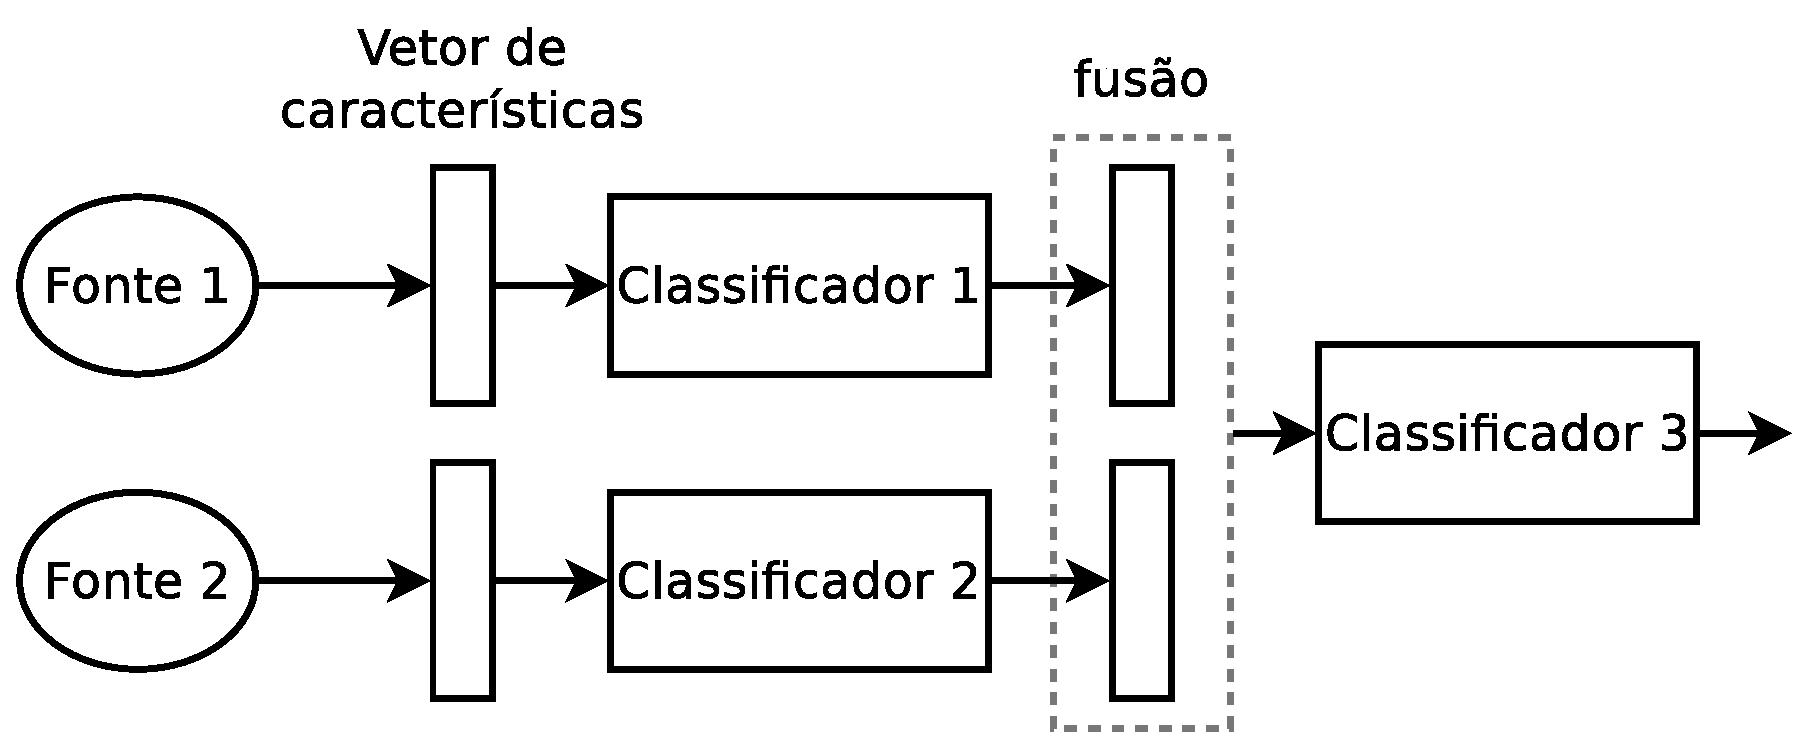
\includegraphics[width=0.95\linewidth]{images/fusion-late.eps}
    \caption{Late fusion (Fonte: Autor)}%kreiss2019pifpaf %OpenPifPaf
    \label{fig:fusion-late}
    \end{figure} 
\end{frame}

%%%%%%%%%%%%%%%%%%%%%%%%%%%%%%%%%%%%%%%%%%%%%%%%%%%%%%%%%%%%%%%%%%%%%%%%%%%%%%%%
\begin{frame}
    \frametitle{Valiação cruzada}
    \begin{figure}[h!]
    \centering
    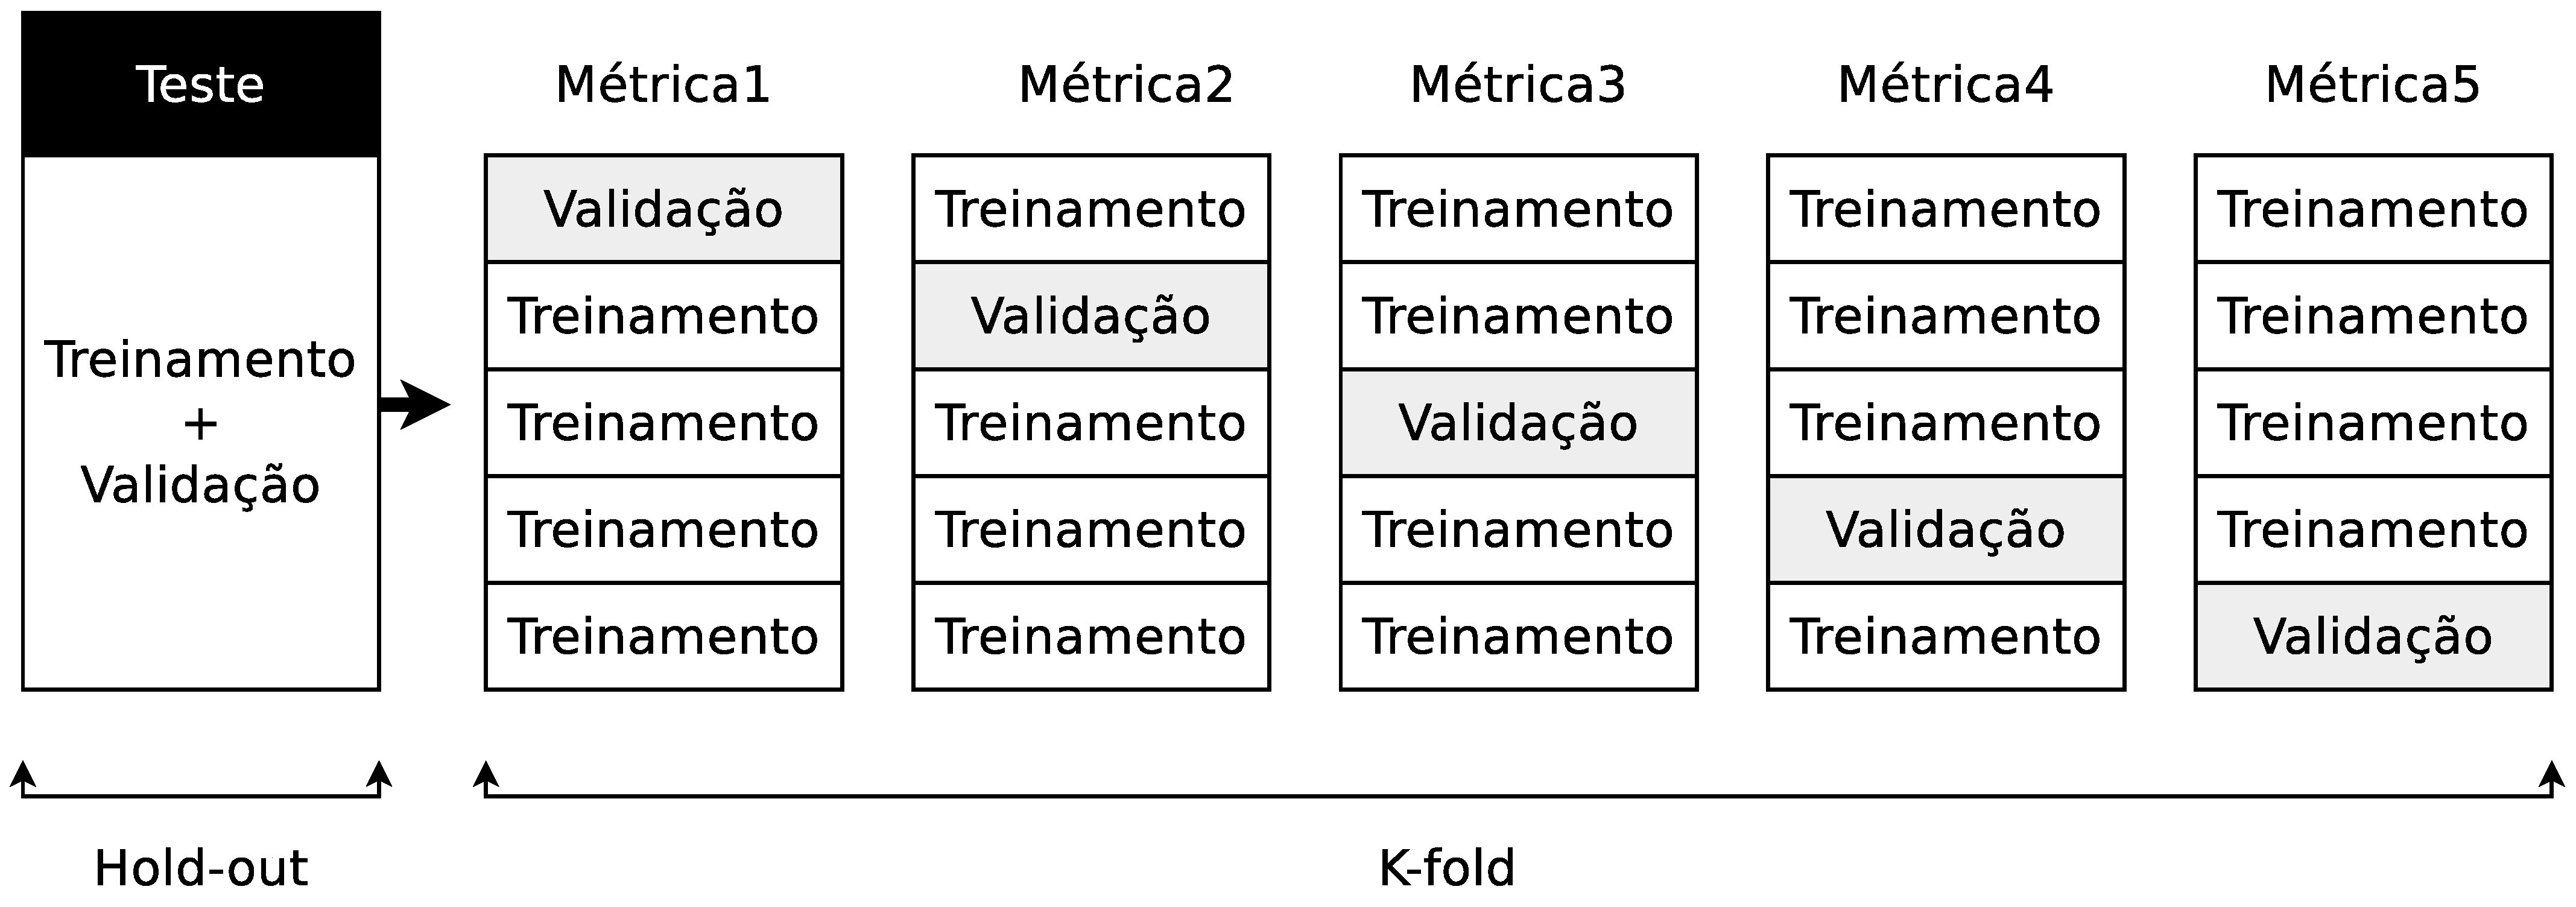
\includegraphics[width=0.95\linewidth]{images/kfold.eps}
    \caption{K-fold (Fonte: Autor)}%kreiss2019pifpaf %OpenPifPaf
    \label{fig:Kfold}
    \end{figure} 
\end{frame}
